% ----------------------------------------------------------
% REVISÃO DA LITERATURA
% ----------------------------------------------------------
\chapter{Revisão da Literatura}
Nesta capítulo buscamos explicitar conceitos e informações relevantes para o desenvolvimento da nossa proposta de solução \emph{estagiei}, um \emph{website} de vagas de estágio.
\begin{comment}
Todos trabalhos devem possuir a revisão de literatura onde são abordados os estudos feitos com base da literatura (livros, artigos acadêmicos, publicações em periódicos), todos elementos devem ser referenciados por citações.

Diversas referencias utilizadas nesse modelo não deveriam ser utilizadas diretamente em um trabalho acadêmico, mas estão aqui para demonstrar de forma mais clara alguns pontos importantes sobre desenvolvimento de projetos

Cada parágrafo da revisão de literatura deve apresentar uma ideia com base em uma referencia 

Copiar e colocar é plágio. Exceto em casos muito específicos onde utilizamos a citação direta você deve escrever com suas palavras (seu entendimento, parafrasear) o que os autores escreveram na publicação original

Não são abordados aqui itens técnicos que normalmente são vistos em disciplinas anteriores do curso (UML, banco de dados, metodologias de gerenciamento de projeto etc...), esses elementos podem receber citações nos outros capítulos do trabalho. Essa regra não se aplica aos trabalhos de pós graduação quando o tema estiver relacionado a conceitos técnicos.

\end{comment}


% ----------------------------------------------------------
% ESTÁGIO
% ----------------------------------------------------------
% ----------------------------------------------------------
% ESTÁGIO
% ----------------------------------------------------------
\section{Estágio}
Nesta seção são apresentados os principais elementos do estágio: sua definição, tipos e carga horária seguindo o estabelecido na legislação brasileira.
\subsection{Definição}
De acordo com a lei nº 11.788, de 25 de setembro de 2008, define-se estágio da seguinte forma:
\begin{quoting}[rightmargin=0cm,leftmargin=4cm]
	\begin{SingleSpace}
	{\footnotesize
	Art. 1º  Estágio é ato educativo escolar supervisionado, desenvolvido no ambiente de trabalho, que visa à preparação para o trabalho produtivo de educandos que estejam freqüentando o ensino regular em instituições de educação superior, de educação profissional, de ensino médio, da educação especial e dos anos finais do ensino fundamental, na modalidade profissional da educação de jovens e adultos. \cite{leiestagio}
	}
	\end{SingleSpace}
\end{quoting}

Portanto, o estágio se trata de uma fase intermediária entre os estudos e a entrada no mercado de trabalho, paralelamente ao primeiro, de acordo com as características da modalidade de ensino, projeto pedagógico e situação do estudante.

\subsection{Tipos de estágio}
Os estágios podem ser obrigatórios ou não-obrigatórios, dependendo do que foi previsto no projeto pedagógico do curso no qual o estudante está matriculado. O estágio do tipo obrigatório se caracteriza pelo requisito de cumprimento de uma determinada quantidade de horas estágio, juntamente com a aprovação nas disciplinas do curso, para a obtenção de diploma. O estágio não-obrigatório é opcional e as horas cumpridas são acrescidas às carga obrigatória do curso. \cite{leiestagio}

\subsection{Carga horária}
O estágio não é regido pela \ac{clt}, assim possui sua própria especificação de jornada e carga horária. De acordo com o Art. 10 \cite{leiestagio}, a jornada do estágio é definida em um acordo entre a escola e a empresa, ressaltando que não pode ultrapassar:
\begin{quoting}[rightmargin=0cm,leftmargin=4cm]
	\begin{SingleSpace}
	{\footnotesize
	I – 4 (quatro) horas diárias e 20 (vinte) horas semanais, no caso de estudantes de educação especial e dos anos finais do ensino fundamental, na modalidade profissional de educação de jovens e adultos;\\II – 6 (seis) horas diárias e 30 (trinta) horas semanais, no caso de estudantes do ensino superior, da educação profissional de nível médio e do ensino médio regular.\\§ 1°  O estágio relativo a cursos que alternam teoria e prática, nos períodos em que não estão programadas aulas presenciais, poderá ter jornada de até 40 (quarenta) horas semanais, desde que isso esteja previsto no projeto pedagógico do curso e da instituição de ensino. \\§ 2°  Se a instituição de ensino adotar verificações de aprendizagem periódicas ou finais, nos períodos de avaliação, a carga horária do estágio será reduzida pelo menos à metade, segundo estipulado no termo de compromisso, para garantir o bom desempenho do estudante.\cite{leiestagio}
	}
	\end{SingleSpace}
\end{quoting}

Nota-se que a carga horária dos estágios tentam ser de tal forma que o estudante tenha condições mínimas de realizar o estágio e ainda conseguir frequentar as aulas de modo apropriado.

% ----------------------------------------------------------
% SPA (SINGLE PAGE APPLICATION)
% ----------------------------------------------------------
\section{Single-page Application (SPA)}
\Gls{spa} é uma implementação de aplicação web que carrega uma única página, um único arquivo do tipo \ac{html}, então de modo dinâmico modifica e atualiza o conteúdo da página de acordo com as ações do usuário, resultando em ganho de performance e melhor experiência de usuário. \cite{spamozilla}

Em uma \ac{spa} toda a codificação \ac{html}, JavaScript e \acs{css} é carregada de uma vez logo no primeiro acesso ou os recursos são recuperados (carregados) e incorporados à página conforme a necessidade, apenas o que for necessário, geralmente em resposta à interação do usuário \cite{wikispa}, como ilustrado na \autoref{spa-lifecycle}.

\begin{figure}[H]
	\centering
	\caption{\label{spa-lifecycle}Ciclo de vida: página web tradicional X \acs{spa}}
	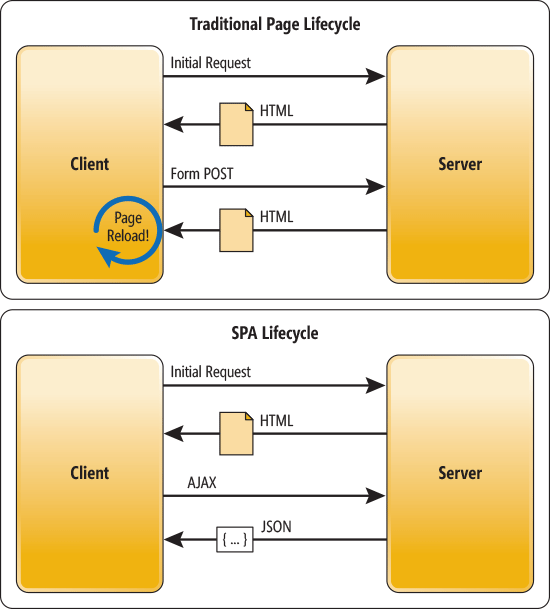
\includegraphics[width=0.50\textwidth]{../imagens/lit-spa-lifecycle.png}
	\fonte{\cite{fig_spa_lifecycle}}
\end{figure}

% ----------------------------------------------------------
% API REST
% ----------------------------------------------------------
%\section{Application Programming Interface (API)} %REST
\Gls{api}, Interface de Programação de Aplicativos, é um sistema intermediário de mediação que permite a comunicação entre outros sistemas/softwares/aplicações a partir de um conjunto de protocolos e definições, ou seja,
\begin{quoting}[rightmargin=0cm,leftmargin=4cm]
	\begin{SingleSpace}
		{\footnotesize APIs funcionam como se fossem contratos, com documentações que representam um acordo entre as partes interessadas. Se uma dessas partes enviar uma solicitação remota estruturada de uma forma específica, isso determinará como a aplicação da outra parte responderá.\cite{redhat_api}}
	\end{SingleSpace}
\end{quoting}
Essa comunicação possibilita uma integração entre produtos e serviços sem que seus desenvolvedores conheçam como o software alheio foi feito, basta saberem as regras para requisitar uma informação e como tratar a resposta. É certo que há formas de incluir segurança no tráfego de informações, essencialmente através do gerenciamento da \ac{api} com gateways \cite{redhat_api}. Desde modo, podemos entender \ac{api} como
\begin{quoting}[rightmargin=0cm,leftmargin=4cm]
	\begin{SingleSpace}
		{\footnotesize [...] um mediador entre os usuários ou clientes e os recursos ou serviços web que eles querem obter. As APIs também servem para que organizações compartilhem recursos e informações e, ao mesmo tempo, mantenham a segurança, o controle e a obrigatoriedade de autenticação, pois permitem determinar quem tem acesso e o que pode ser acessado. \cite{redhat_api}}
	\end{SingleSpace}
\end{quoting}

\subsection{API REST}
\Gls{rest} é um estilo de arquitetura com um conjunto de restrições \cite{redhat_apirest}. Uma \ac{api} que segue todas as seis restrições é chamada de \gls{apirestful} \cite{royfielding}. Como não se trata de um protocolo específico, não há um padrão de implementação das restrições \ac{rest}, que seguem:
\begin{quoting}[rightmargin=0cm,leftmargin=4cm]
	\begin{SingleSpace}
		{\footnotesize 
			\begin{itemize}
				\item Arquitetura cliente-servidor: a arquitetura \ac{rest} é composta por clientes, servidores e recursos. Ela lida com as solicitações via \acs{http}.
				\item Sem monitoração de estado: nenhum conteúdo do cliente é armazenado no servidor entre as solicitações. Em vez disso, as informações sobre o estado da sessão são mantidas com o cliente.
				\item Capacidade de cache: o armazenamento em cache pode eliminar a necessidade de algumas interações entre o cliente e o servidor.
				\item Sistema em camadas: as interações entre cliente e servidor podem ser mediadas por camadas adicionais. Essas camadas podem oferecer recursos extras, como balanceamento de carga, caches compartilhados ou segurança.
				\item Código sob demanda (opcional): os servidores podem ampliar a funcionalidade de um cliente por meio da transferência de códigos executáveis.
				\item Interface uniforme: essa restrição é essencial para o design de \gls{apirestful} e inclui quatro vertentes:
				\subitem -Identificação de recursos nas solicitações: os recursos são identificados nas solicitações e separados das representações retornadas para o cliente.
				\subitem -Manipulação de recursos por meio de representações: os clientes recebem arquivos que representam recursos. Essas representações precisam ter informações suficientes para permitir a modificação ou exclusão.
				\subitem -Mensagens autodescritivas: cada mensagem retornada para um cliente contém informações suficientes para descrever como ele deve processá-las.
				\subitem -Hipermídia como plataforma do estado das aplicações: depois de acessar um recurso, o cliente \ac{rest} pode descobrir todas as outras ações disponíveis no momento por meio de hiperlinks. \cite{redhat_api}
			\end{itemize}
			}
	\end{SingleSpace}
\end{quoting}
Caso não seja o objetivo criar uma \gls{apirestful}, as restrições da arquitetura \ac{rest} podem ser implementadas conforme a necessidade, tornando o desenvolvimento da \ac{api} mais fácil por não haver exigências rígidas, como um formato específico para a informação de resposta às requisições via \ac{http} ou \ac{https}, por exemplo \cite{redhat_apirest}. Porém, ainda que não haja uma obrigatoriedade, o formato \ac{json} é o mais utilizado, pois é de fácil manipulação, organização e inteligível para pessoas e máquinas.

% ---
